% !TeX root = ../../main.tex
% Add the above to each chapter to make compiling the PDF easier in some editors.

\section{Inside-Outside Guidance}\label{ord:ch3:sec4}

Another approach for interactive segmentation is the \gls{iog} method, introduced in \cite{Zha20-IOG}.
The concept of this state-of-the-art method is strongly based on the previously introduced \gls{dextr} method \cite{Man18-DEXTR}.

\subsection{Basic Concept}\label{ord:ch3:sec4:subsec1}
% User Clicks - Workflow
The user interaction of the \gls{iog} method requires three user clicks executed in two steps.
First, the user has to create a tight bounding box around the object of interest. 
The creating of the bounding box may be counted as two user clicks on the background.
However, in practice the bounding box is mostly drawn by a stroke which is more intuitive.
Second, the user has to click once on the center of the object, which is represented as foreground click. 
The described workflow is illustrated in Figure \ref{fig:ch3:sec4:iog_user_clicks}.
Further, the user clicks are processed and an object mask is predicted by a \gls{dl} model.

% Naming of the method
% two-fold
The user provides high level guidance on the foreground and background, representative for the inside and outside region of the object.
On the one hand, this guidance is based on the bounding box that defines the background.
So, everything outside the bounding box does not belong to the object, this is described as \textit{outside} guidance.
On the other hand, the foreground click provides explicit guidance, where the object is located.
This is referred to as \textit{inside} guidance.
It also results that the object is always inside the bounding box, therefore, the background clicks also provide a kind of \textit{inside} guidance. 
These two types of guidance are the namesake of the method \glsentryfull{iog}.

% Advantage over DEXTR
Zhang \etal claim, that their way to set user clicks has two advantages compared to the way to set user clicks in other interactive methods as \gls{dextr}.
First, setting of extreme points may be confusing and misleading, as they may be located very close to each other, depending on the orientation of the object.
Second, if the object of interest contains a hole (\eg a donut) or another object is in front of it, \gls{dextr} cannot provide a robust guidance.
In contrast, the variable position of the foreground click in \gls{iog} enables a more robust guidance even for special object scenarios \cite{Zha20-IOG}.

\begin{figure}
	\centering
	\begin{subfigure}[b]{0.3\textwidth}
		\centering
		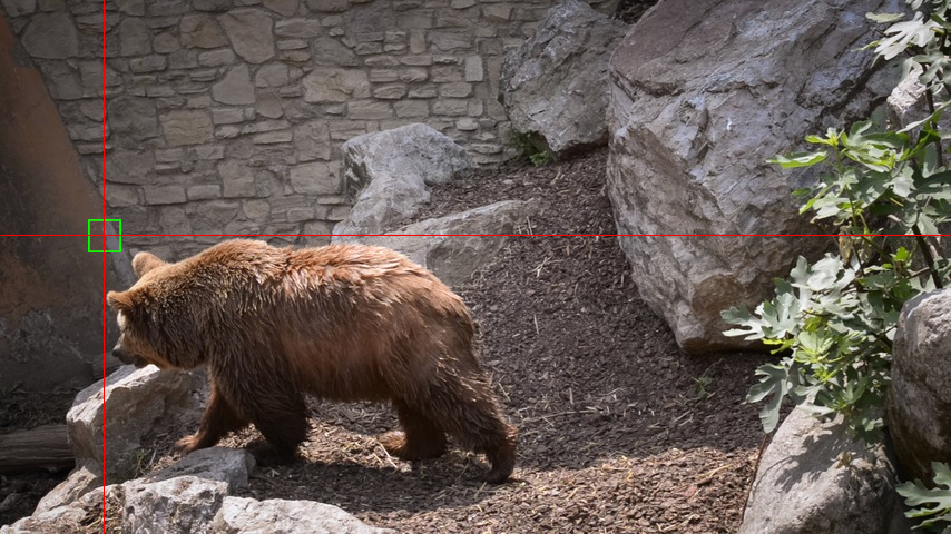
\includegraphics[width=\textwidth]{figures/chap34_bear_2.png}
		\caption{First background click.}
		\label{fig:ch3:sec4:iog_workflow_1}
	\end{subfigure}
	\hfill
	\begin{subfigure}[b]{0.3\textwidth}
		\centering
		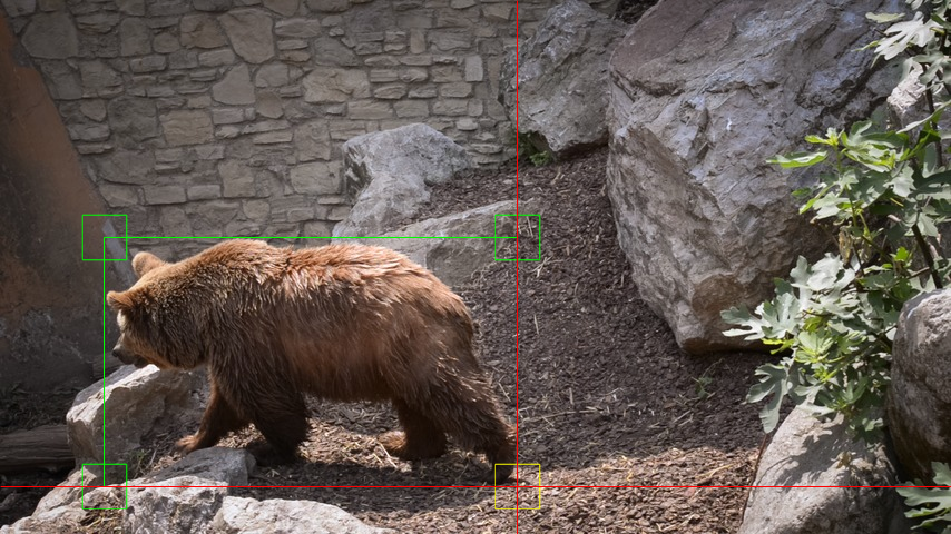
\includegraphics[width=\textwidth]{figures/chap34_bear_3.png}
		\caption{Second background click.}
		\label{fig:ch3:sec4:iog_workflow_2}
	\end{subfigure}
	\hfill
	\begin{subfigure}[b]{0.3\textwidth}
		\centering
		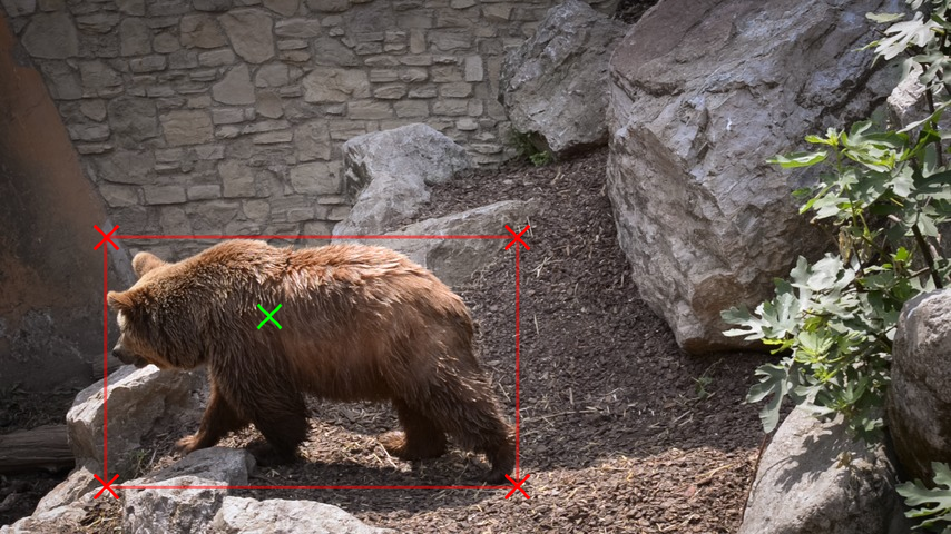
\includegraphics[width=\textwidth]{figures/chap34_bear_5.png}
		\caption{Foreground click.}
		\label{fig:ch3:sec4:iog_workflow_3}
	\end{subfigure}
	\caption[IOG User Interaction]{
		Shown is the workflow to perform the user interaction required for the \gls{iog} method.
		First, a bounding box is spanned by setting two background clicks.
		Last, the foreground click is set.
		All used points are visualized with a cross, background points in red and the foreground point in green, while the contour of the bounding box is drawn in red.
	} 
	\label{fig:ch3:sec4:iog_user_clicks}
\end{figure}

\subsection{Model Input and Representation of User Clicks}\label{ord:ch3:sec4:subsec2}

Similar to the \gls{dextr} method, the background clicks form a bounding box, which is enlarged by  $p_{{box}} = 10 $ \Unit{px}.
The image is cropped based on the enlarged bounding box and resized to the size of $512 \times 512$ \Unit{px}, if necessary zero padding is applied.

The bounding box is formed by the two background points, that are diagonal corners points (top-left and bottom-right or bottom-left and top-right).
Based on these two points, the other two corner points are derived, which provides four background points for the price of two.
As in the \gls{dextr} processing, the fore- and background clicks are converted into points on two separate heatmaps.
To highlight the user points a 2D Gaussian with $ \sigma = 10 $ is centered around each click (see Equation \ref{equ:gauss} or Figure \ref{fig:ch3:sec3:gauss_centered_point}).

The two heatmaps have the size of $512 \times 512$ \Unit{px} and are concatenated with the \Gls{rgb} image.
This results in the five-channel input for the \gls{iog} model, which is explanatory illustrated in Figure \ref{fig:ch3:sec4:model_input_channels}.

%TODO plots add crosses to cropped RGB image
\begin{figure}
	\centering
	\begin{subfigure}[b]{0.3\textwidth}
		\centering
		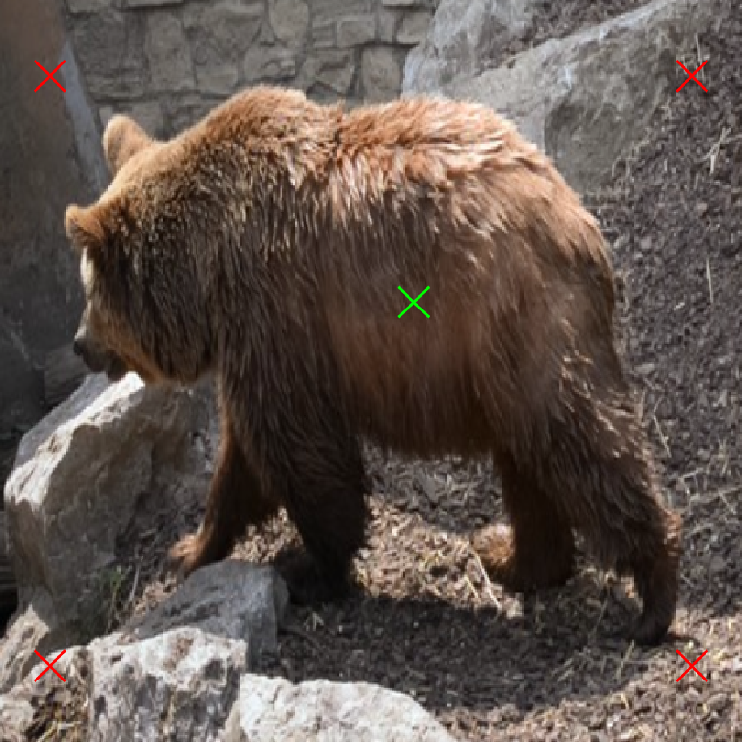
\includegraphics[width=\textwidth]{figures/chap34_channel_rgb.png}
		\caption{RGB image cropped based on the bounding box (three channels).}
		\label{fig:ch3:sec4:rgb_channel}
	\end{subfigure}
	\hfill
	\begin{subfigure}[b]{0.3\textwidth}
		\centering
		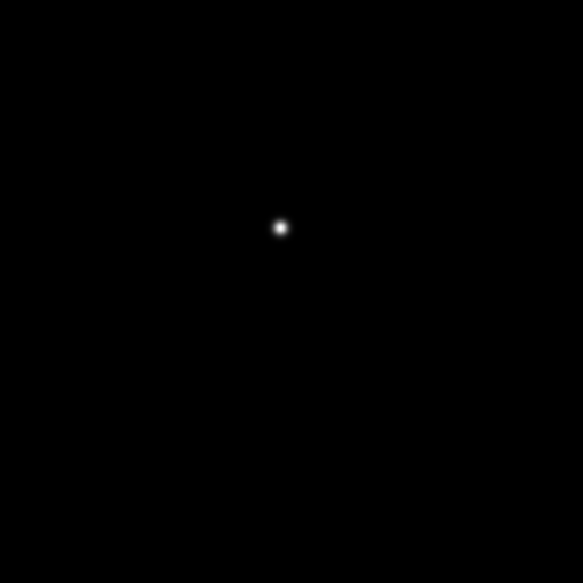
\includegraphics[width=\textwidth]{figures/chap34_channel_fg.png}
		\caption{Foreground heatmap with one foreground point (one channel).}
		\label{fig:ch3:sec4:fg_channel}
	\end{subfigure}
	\hfill
	\begin{subfigure}[b]{0.3\textwidth}
		\centering
		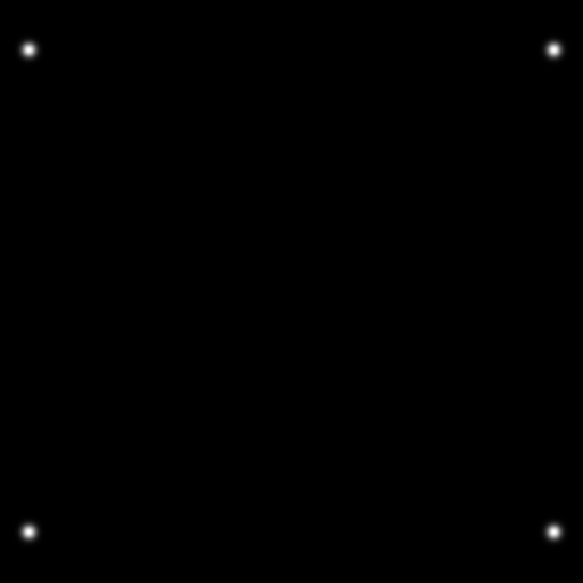
\includegraphics[width=\textwidth]{figures/chap34_channel_bg.png}
		\caption{Background heatmap with four background points (one channel).}
		\label{fig:ch3:sec4:bg_channel}
	\end{subfigure}
	\caption[Five-channel IOG model input]{
		Representation of the separate channels from the five-channel input for the \gls{iog} model.
		All channels have the spatial dimension of $512 \times 512$ \Unit{px}.
		The user points in the foreground and background heatmaps are enforced with a 2D Gaussian.
	} \label{fig:ch3:sec4:model_input_channels}
\end{figure}

\subsection{Architecture}\label{ord:ch3:sec4:subsec3}

The model architecture used for the \gls{iog} method is based on the encoder-decoder architecture and special structure for layer fusion.
The encoder-decoder network is titled as \textit{CoraseNet}, while the structure for layer fusion is referred to as \textit{FineNet}.
An illustration of the complete architecture is given in Figure \ref{fig:ch3:sec4:arch}.


\subsubsection{CoarseNet}
The CoarseNet consists out of multiple components: encoder network, decoder network, \gls{psp}-module and skip connections. The CoarseNet is built upon the \gls{dextr} method, therefore they partially share the same architectural components.

As in the \gls{dextr} architecture, the encoder network is represented by the ResNet-101 \cite{He16-ResNet}, followed by a \gls{psp} module.
%The ResNet is implemented without the head of fully connected layers. It contains four ResNet blocks and the fourth block outputs 2048 feature maps of the size $32 \times 32$ \Unit{px}.
% As in \gls{dextr} a \gls{psp}-module is applied after the backbone to gain more contextual information.
The output of the \gls{psp}-module is a coarse prediction with the spatial dimension of  $32 \times 32$ \Unit{px} containing 512 feature maps. 

From this onward the decoder network starts the upsampling process.
The decoder network is built upon a reversed, simplified version of the encoder architecture. % , that consists out of four residual blocks.
Therefore, the decoder network is based on four blocks, in order to regain the original input size of  $512 \times 512$ \Unit{px}.
Further, three skip connection are applied and establish a connection in between the four resiudual blocks of the encoder and decoder network, as visualized in Figure \ref{fig:ch3:sec4:arch}.
Here with each of these skip connections also a convolution layer with batchnorm \cite{SS15-Batchnorm} and activation function are applied.
A characteristic of this architecture is the fusion of information from different network components.

\begin{figure}
	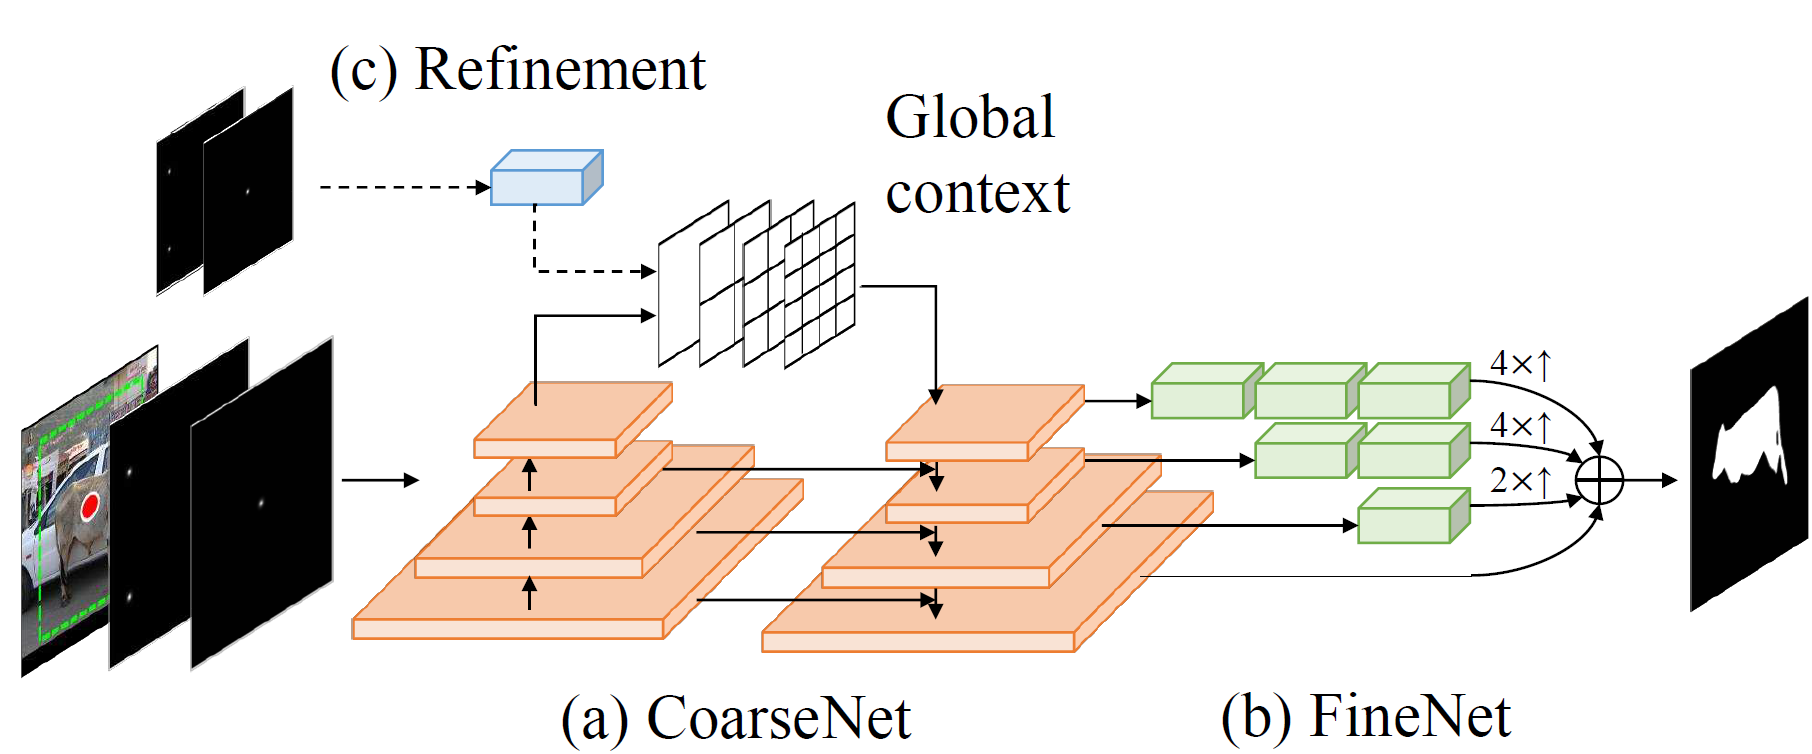
\includegraphics[width=\linewidth]{figures/chap34_iog_arch.png}
	\caption[IOG Architecture]{		
		Architecture of the \gls{iog} model.
		On the left the model input is visualized as in Figure \ref{fig:ch3:sec4:model_input_channels}.
		The CoarseNet is marked by (a) and shows the encoder and decoder network with the skip connections and the \gls{psp} module.
		The FineNet is marked by (b) and represents the four stream fusion structure.
		It can be seen, that the single streams origin from different levels of the decoder network.
		In order to obtain a common spatial dimension for concatenation $ \oplus $, the streams differ in their processing.
		As final prediction a binary object mask is shown.
		The lightweight-branch for refinement is marked with (c).
		\copyright 2020 IEEE. Reprinted by permission from \cite{Zha20-IOG}.
	}
	\label{fig:ch3:sec4:arch}
\end{figure}

\subsubsection{FineNet}
The FineNet consists of a four-stream fusion structure.
The four streams originate from the four levels of the decoder network and, therefore, process feature maps of various sizes (see Figure \ref{fig:ch3:sec4:arch}).
Each stream processes and upsamples the feature maps by a descending number of bottleneck processing blocks.
The streams reconstruct the feature maps to the final spatial dimension of $512 \times 512$ \Unit{px}.
In the end the four streams are concatenated and pass through a last bottleneck block.
To the final output a sigmoid is applied, which results in a probability map as prediction of the \gls{iog} network.

The author justifies the application of these different components by showing their effect in an ablation study \cite{Zha20-IOG}.
The settings for training the \gls{iog} network are identical to the \gls{dextr} network.

\subsection{Refinement}\label{ord:ch3:sec4:subsec4}

To perform refinement in the \gls{iog} method, users set an additional click on the largest fore- or background region that was predicted wrongly.
Identically to the \gls{dextr} method, refinement may be performed iteratively and each refinement click triggers a model execution.
However, in contrast to \gls{dextr} the refinement of the \gls{iog} method does not require the execution of the complete model.

The integration in the existing architecture is realized as follows.
New heatmaps for fore- and background are created with the original clicks and the refinement clicks.
These two heatmaps are combined into a two-channel input, which is processed in a so called lightweight-branch.
This lightweight-branch consists out of five convolutional layers, that perform the downsampling.
The output of this branch is combined with the output of the initial iteration from the encoder network and forwarded to the \gls{psp} module as shown in Figure \ref{fig:ch3:sec4:arch}.
This means that the computationally expensive encoder must only be executed once for the initial prediction.
From the \gls{psp} module onwards the model is executed normally.

Hence, the encoder network does not require a new execution and the execution of the model time is decreased.
Zhang \etal state, that the usage of the lightweight-branch performs better than directly adding the refinement click into the normal five-channel input.

% TODO plots use an example where the initial prediction actually fails and the refinement succeeds.
\begin{figure} 
	\centering
	\begin{subfigure}[b]{0.45\textwidth}
		\centering
		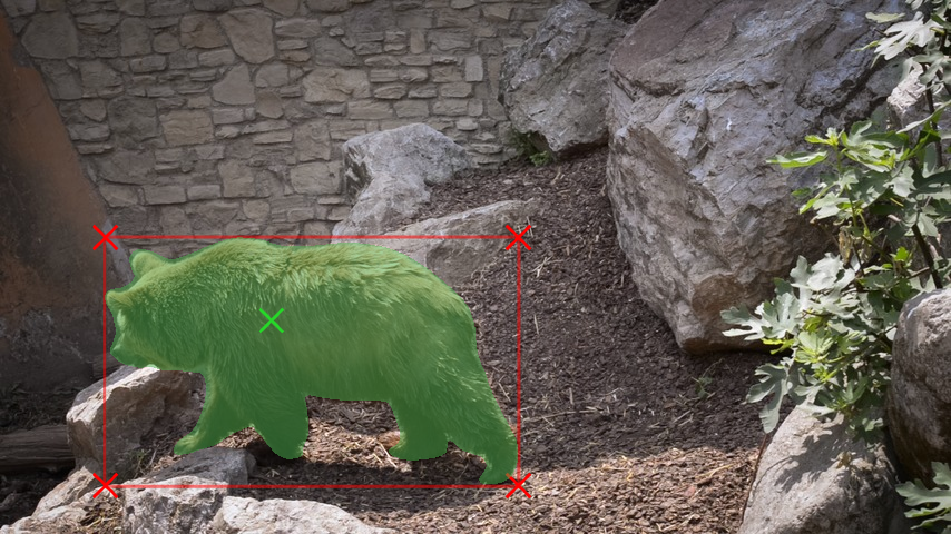
\includegraphics[width=\textwidth]{figures/chap34_bear_6.png}
		\caption{Initial segmentation result.}
		\label{fig:ch3:sec4:refinement_1}
	\end{subfigure}
	\hfill
	\begin{subfigure}[b]{0.45\textwidth}
		\centering
		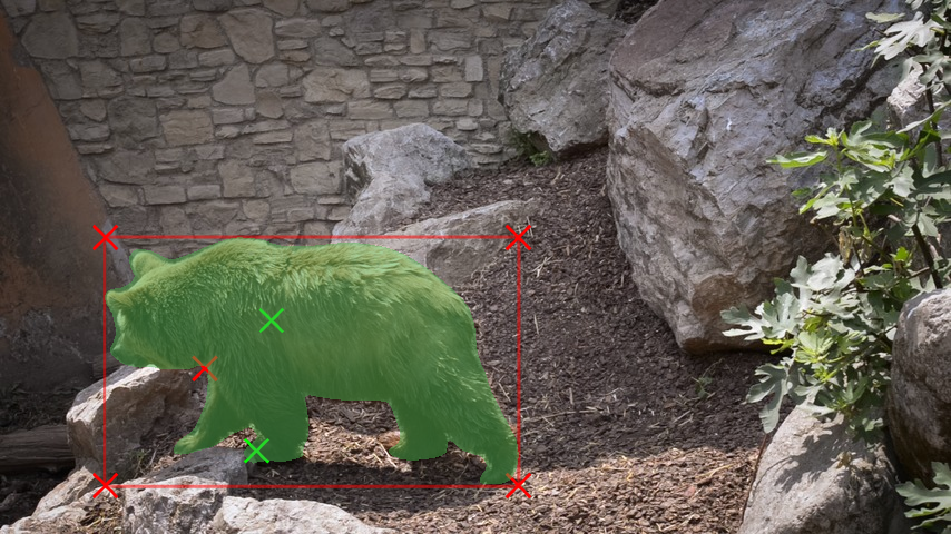
\includegraphics[width=\textwidth]{figures/chap34_bear_8.png}
		\caption{Refinement segmentation result.}
		\label{fig:ch3:sec4:refinement_2}
	\end{subfigure}
	\caption[IOG Refinement]{
		On the left is the initial result with the normal amount of clicks. 
		On the right is the results of two refinement iterations with one additional refinement click on the foreground and one on the background.
	} \label{fig:ch3:sec4:refinement}
\end{figure}


\subsection{Performance}\label{ord:ch3:sec4:subsec5}

An overview of interactive segmentation methods is presented in Table \ref{tab:ch2:interactive-stae-of-the-art}.
It can be seen that the \gls{iog} outperforms other state-of-the-art methods with respect to the number of set points to reach a certain IoU-level and the achieved \gls{iou} at exactly four clicks.

It is assumed that this method especially performs well due the highly connected architecture.
The application of skip connections and the FineNet enable the model to recover local details and prevent the information loss during down- and upsampling process.

Similar to the experiments performed in \cite{Man18-DEXTR}, Zhang \etal also investigate the performance on unseen classes and the generalization capability of the method \Cite{Zha20-IOG}. 
This topic will be continued by the evaluation of other unseen domains in Section \ref{ord:ch5:sec2_generalization_image_domains}.

Zhang \etal also evaluate the performance on dataset with other domains than PASCAL \gls{voc} (\eg Rooftops, CityScapes, or Agricultural-Vision).
Further, it is demonstrated in various setups, that the \gls{iog} method trained on PASCAL \gls{voc} outperforms the \gls{dextr} method or the \textit{Curve-\gls{gcn}}, both trained on the CityScapes dataset.

% TODO plots appendix with various examples of IOG segmentation results?